\chapter{Evaluation}
\label{c:evalu}

In this chapter, we discuss the end-to-end evaluation of our system using the sensor hints of the smartphone and without the sensor hints for our recorded dataset.
Later in this chapter, we discuss the evaluation of our system using a public dataset.

\section{Evaluation dataset}
\label{s:eval}
For collecting the ground truth data we walked along the path of 300 feet at an urban street to record the video with samrtphone.
We record data at different time of the day and at different light condition.
\ref{f:dataset} shows the scene variation of recored video.
The right one is cloudy and the left one is sunny.

\begin{figure}[!ht]
\centering
\subfloat[Sunny] {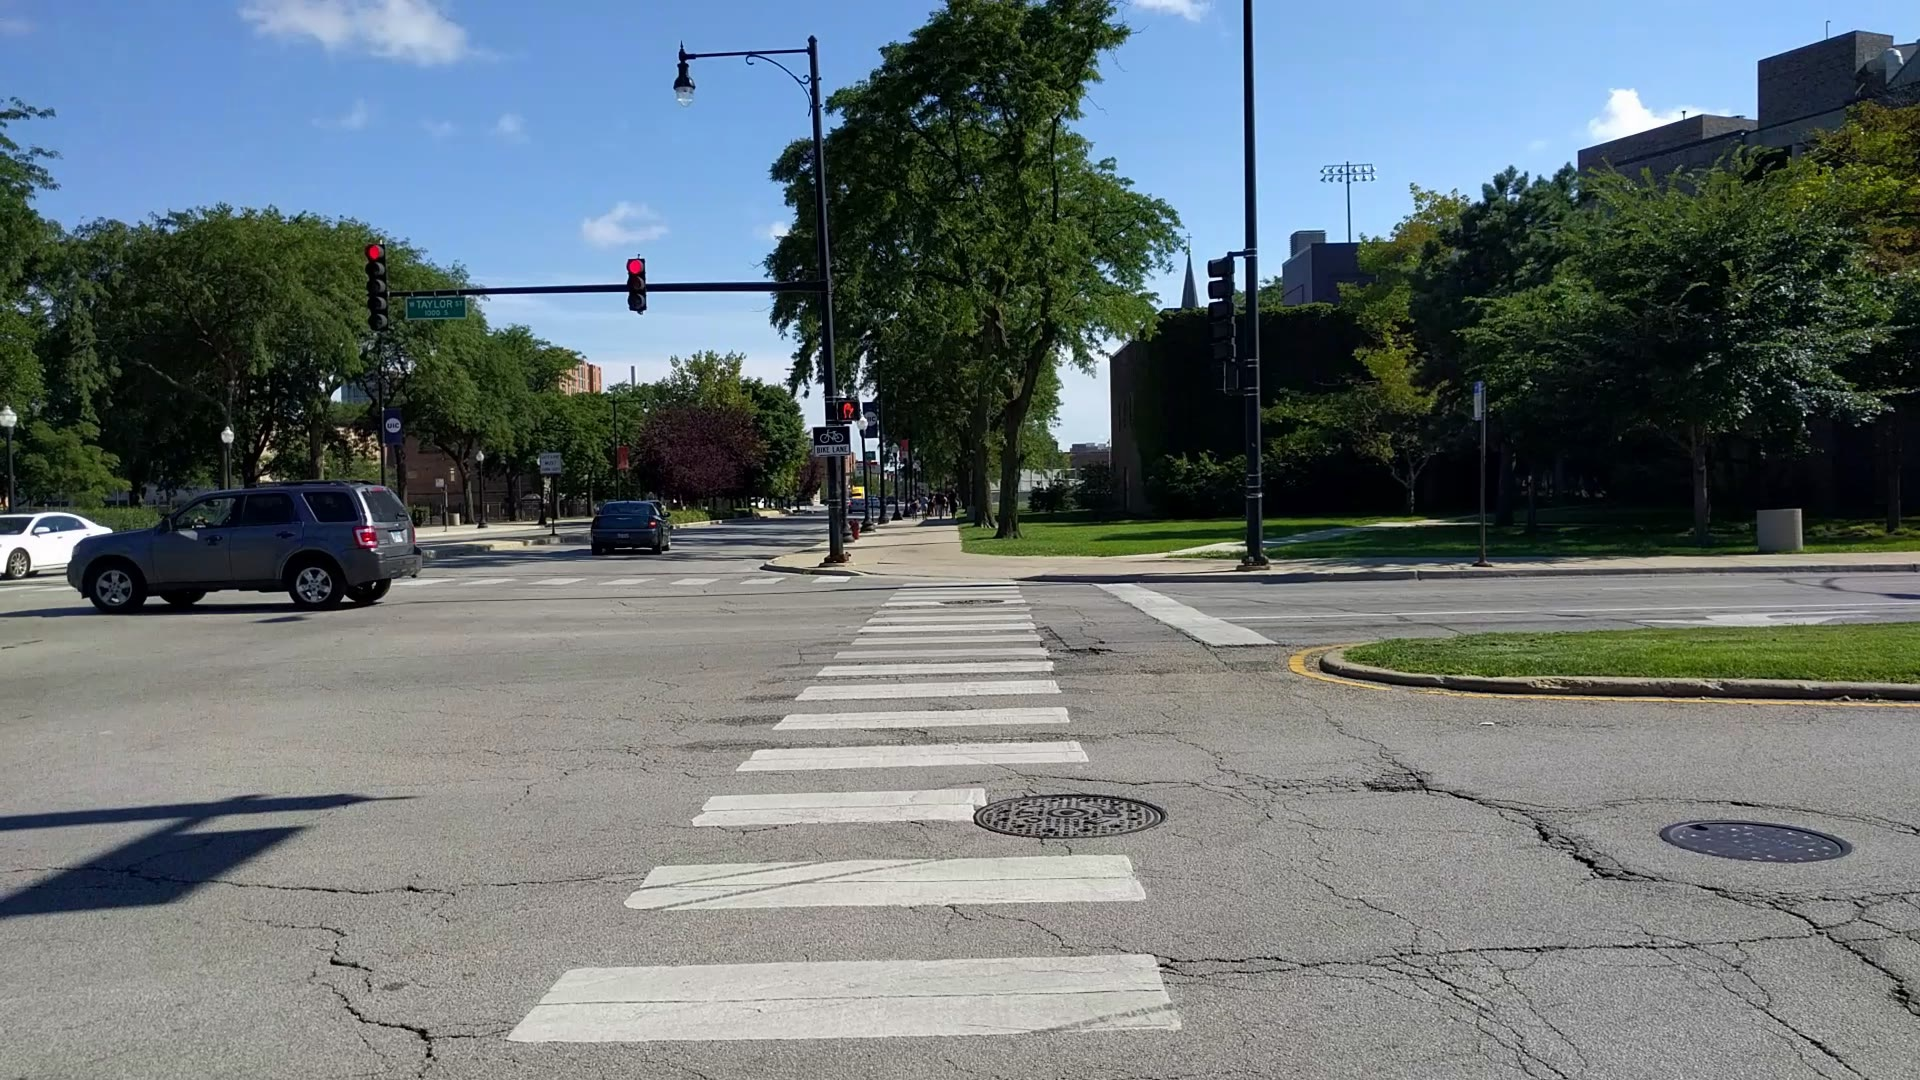
\includegraphics[width=3.1in]{images/sunny.jpg}}
\hfill
\subfloat[Cloudy] {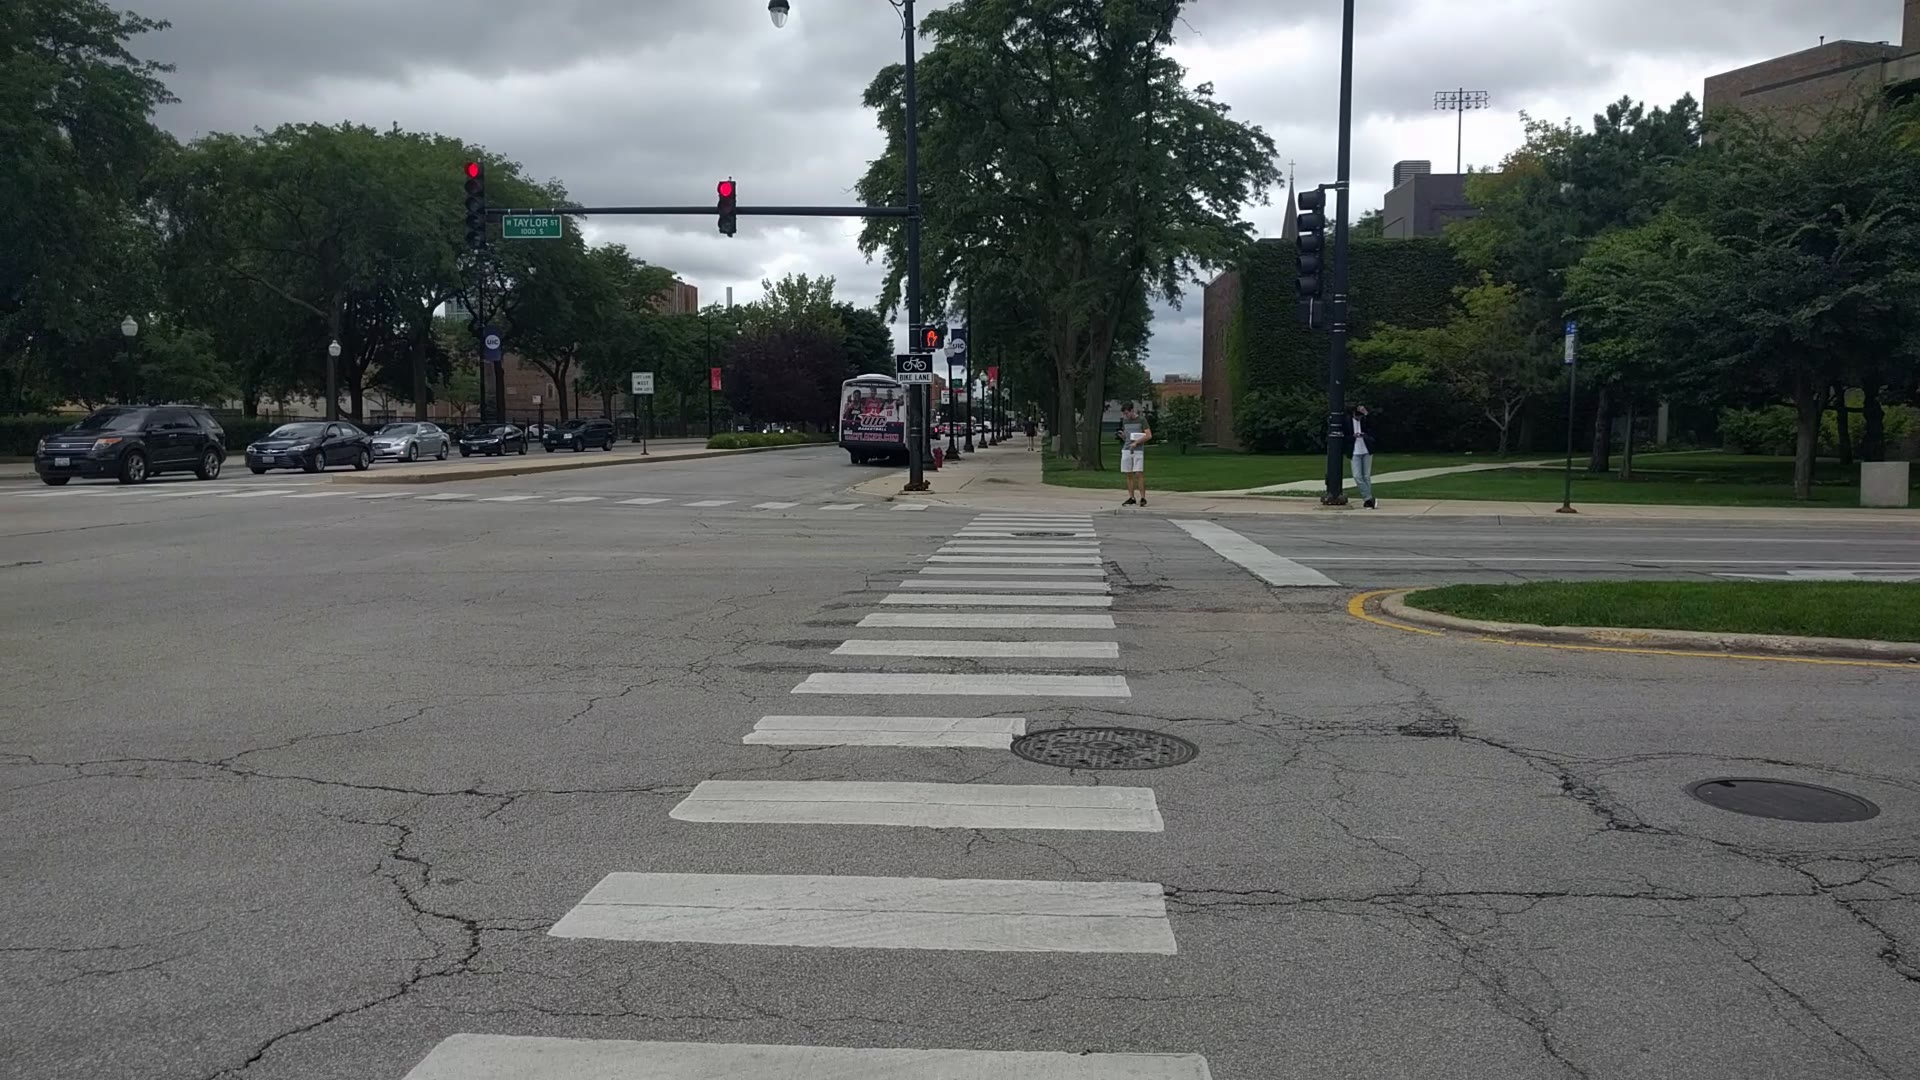
\includegraphics[width=3.1in]{images/cloudy.jpg}}
\caption{Scene variation of recorded video.}
\label{f:dataset}
\end{figure}

\ref{t:dataset} shows the total no of frames, and time duration of our dataset.

\begin{table}[h!]
  \centering
  \caption{Description of the dataset.}
  \label{t:dataset}
  \begin{tabular}{  l  c  r  }
   
    Name & Frame Count & Time Duration \\
    \hline
    Walk with sensor movement-Sunny day & 5905 & 3 mins 16 secs  \\
    Walk with sensor movement-Cloudy day & 6205 & 3 mins 26 secs \\
    Walk regular movement & 6022 & 3 mins 20 secs \\
    Static with sensor movement & 1810 & 1 min \\
    \hline
  \end{tabular}
\end{table}

\section{Annotation}
To measure our system performance quantitatively, we need the ground truth for traffic light.
We annotate the traffic light's position manually at each video frame to get the ground truth.
We remark the traffic light state: red or green and the location of traffic light.

\begin{figure}[h!]
\centering
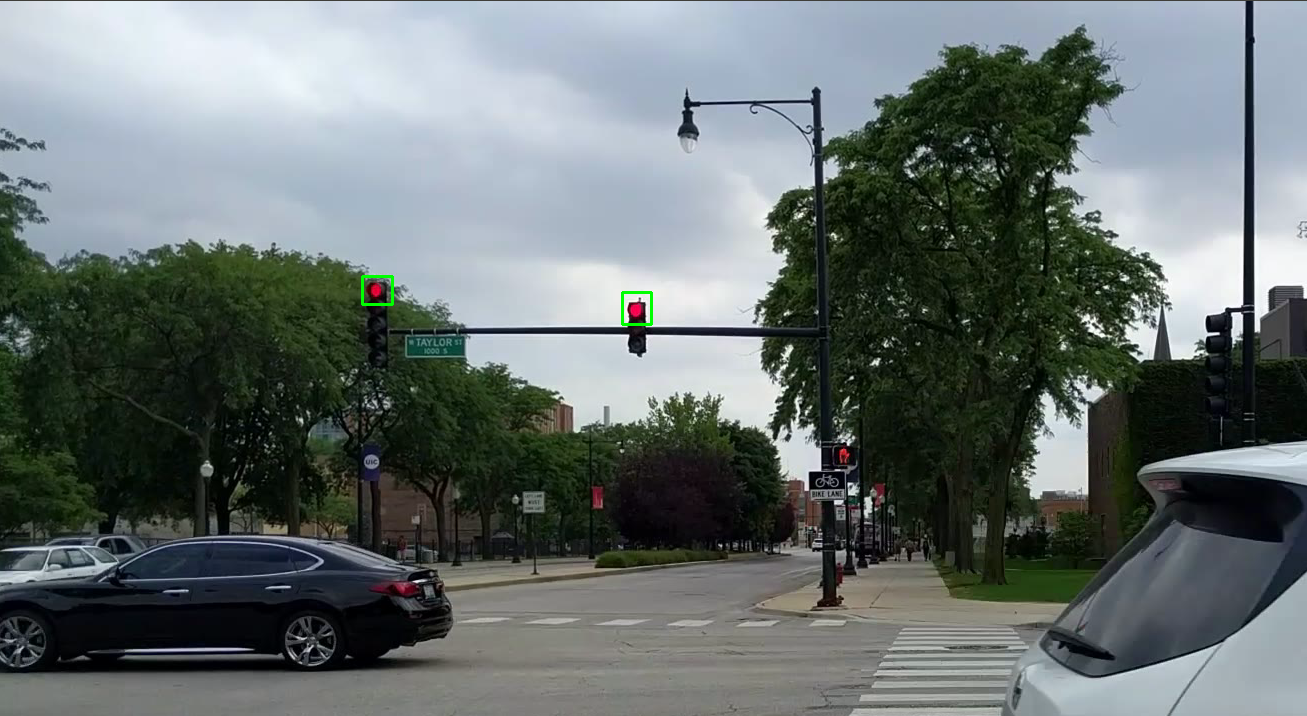
\includegraphics[width=5.2in]{images/annotation.png}
\caption{Interface for manual annotation.}
\label{f:annotate}
\end{figure}

\ref{f:annotate} shows the interface for manual annotation.
The green box gives the location of the traffic light and we annotate 0 for red traffic light and 1 for green.

\section{Computation time}
We collected data at different time of the day as we discussed in \ref{s:eval}.
In this section we discuss the computation time of these datasets with the sensor hint and without it.

\subsection{Computation time for heuristic filter}

We use a heuristic filter to get better traffic light detection as we discuss at \ref{s:filter}.
The computational cost is trivial for this heuristic filter.

\begin{figure}[h!]
\centering
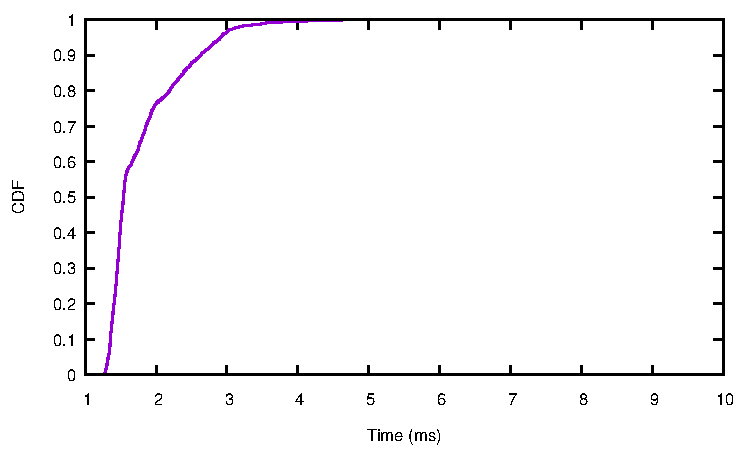
\includegraphics[width=5.2in]{plots/sunny_cdf_filter.pdf}
\caption{CDF of computation time for heuristic filter.}
\label{f:cdf_fil}
\end{figure}

\ref{f:cdf_fil} shows the computation time for the heuristic filter we discuss at \ref{s:filter}.
The computation time depends on the number of circle detected on the frame.
If circle count is high, filtering need for all of these circles, so computation time will be higher.
\ref{f:cdf_fil} shows that the median computation time is 1.5 ms for the filtering. 


\begin{figure}[h!]
\centering
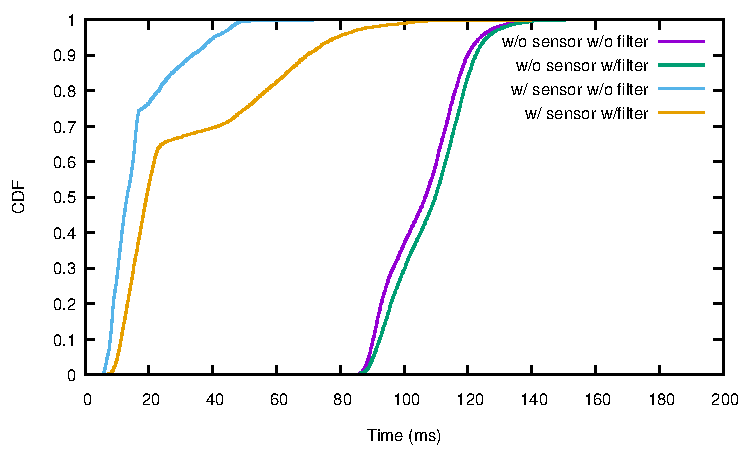
\includegraphics[width=5.2in]{plots/walk_cdf_time.pdf}
\caption{CDF of frame computation time.}
\label{f:cdf_time}
\end{figure}

\subsection{Computation time for video frames}
\ref{f:cdf_time} shows the CDF of the video frame computation time for walking dataset with regular movement, we discuss at \ref{s:eval}.
It shows that the median of the computation time without sensor and any heuristic filter is 106ms.
Wheather, the median of the computation time with sensor and without heuristic filter is 13ms.
We can improve the computation time 8.15x.
The median of the computation time with sensor and heuristic filter is 19ms.
Though we can improve the computation time 5.57x with the filter but it increases the accuracy, which we will describe at section \ref{s:acc}

\begin{figure}[h!]
\centering
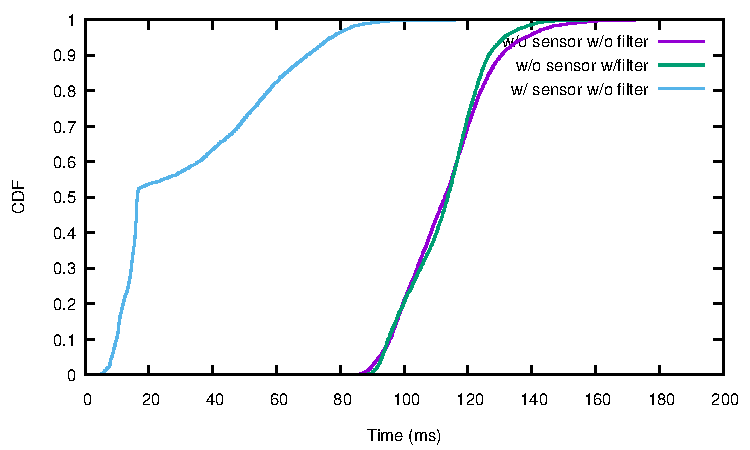
\includegraphics[width=5.2in]{plots/sunny_cdf_time.pdf}
\caption{CDF of frame computation time for walking dataset in sunny weather.}
\label{f:cdf_sunny}
\end{figure}

\ref{f:cdf_sunny} shows the CDF of the video frame computation time for walking dataset with sensor movement at sunny weather.
\ref{f:cdf_sunny} shows that the median computation time without sensor is 107ms and with sensor is 13ms.
So we can improve the computation time 8.23x.

\subsection{Computation time for subpart images}
In section \ref{s:roi}, we discuss the change of region of interest area with the sensor hints.
The failed detection in a subpart images causes to increase the subpart area. 

\begin{figure}[h!]
\centering
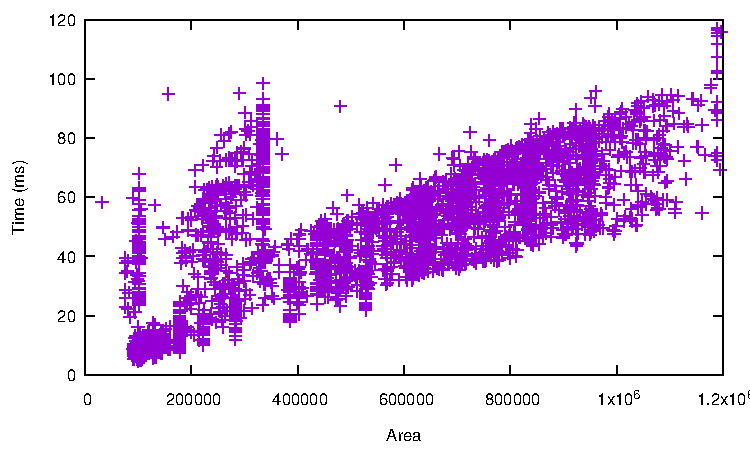
\includegraphics[width=5.2in]{plots/sunny_recarea.pdf}
\caption{Computation time with the increase of the rectangle area.}
\label{f:recarea}
\end{figure}
\ref{f:recarea} shows the computation time with the increase of the subpart area of video frames.
As we can see, when area of subpart images increase computation time is increasing.
At the same area, if the amount of candidate pixels is high or the detected circle count is high, computation time is also varying.

\section{Detection accuracy of our system}
\label{s:acc}
To demonstrate the robustness of the various traffic light scenarios, we recorded video at different lightening condition: cloudy and sunny and at different time of the day.
We walked along the intersection of the street and the route consist of 16 traffic light.

\subsection{Confusion matrix}

\ref{t:con_nocrp} shows a confusion matrix for the traffic light decision when we do not consider the sensor hints of the smartphone.
\ref{t:con_crp} shows the confusion matrix considering the sensor hints in the same dataset.

\begin{table}[h!]
  \centering
  \caption{Confusion Matrix without sensor hints for static movement dataset.}
  \label{t:con_nocrp}
  \begin{tabular}{  l | c | c | r }
   
     & Detected Red & Detected Green &  \\
    \hline
    Actual Red & 828 & 1 & 99.88\% \\
    \hline
    Actual Green & 54 & 509 & 90.41\% \\
    \hline
    & 93.88\% & 98.8\% & 96.05\% \\
    
  \end{tabular}
\end{table}

\begin{table}[h!]
  \centering
  \caption{Confusion Matrix with sensor hints for static movement dataset.}
  \label{t:con_crp}
  \begin{tabular}{  l | c | c | r }
   
     & Detected Red & Detected Green &  \\
    \hline
    Actual Red & 909 & 1 & 99.89\% \\
    \hline
    Actual Green & 36 & 524 & 93.57\% \\
    \hline
    & 96.19\% & 99.81\% & 97.48\% \\
    
  \end{tabular}
\end{table}

These results show that, using the sensor hints our system is more accurate detecting the red light and also false detection of green light is decreasing.

\subsection{Detection and misdetection rate for traffic light}

\ref{f:tp_stat} shows the detection rate for the red and green state of the traffic light.
It shows that using the sensor hints detection rate for red light increases from 86\% to 96\% and for green light, detection rate increases 96\% to 99\%.

\begin{figure}[h!]
\centering
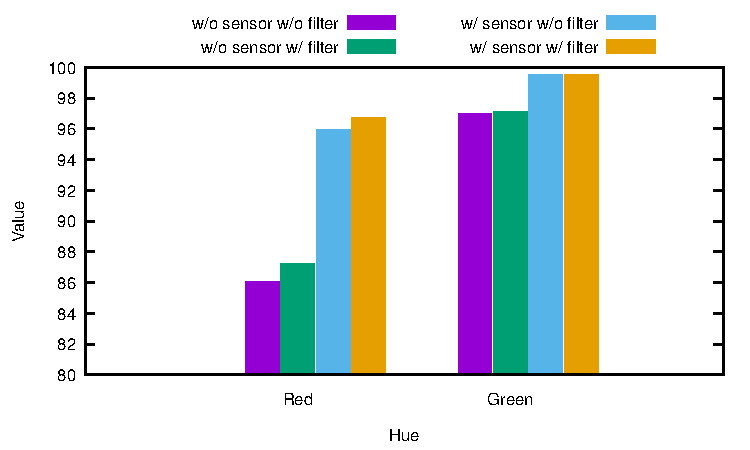
\includegraphics[width=5.2in]{plots/bar_tp.pdf}
\caption{Detection rate for static movement dataset.}
\label{f:tp_stat}
\end{figure}

\ref{f:fp_stat} shows the misdetection rate for the red and green state of traffic light.
Left one is the false positive detection and the right one is the false negative detection for the traffic light detection.

\begin{figure}[!ht]
\centering
\subfloat[] {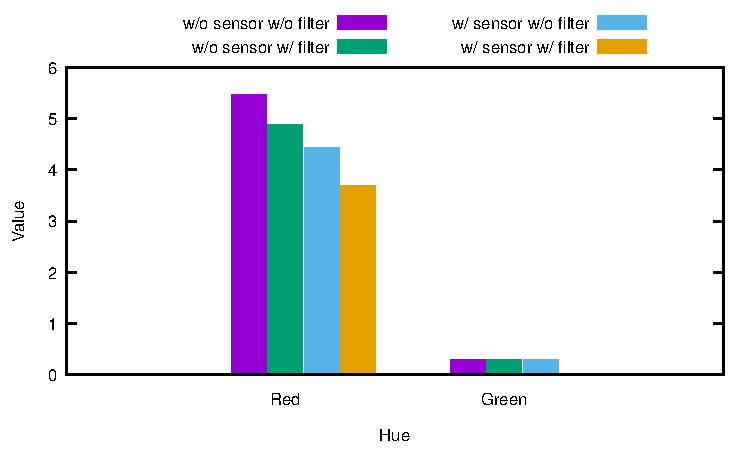
\includegraphics[width=3.1in]{plots/bar_fp.pdf}}
\hfill
\subfloat[] {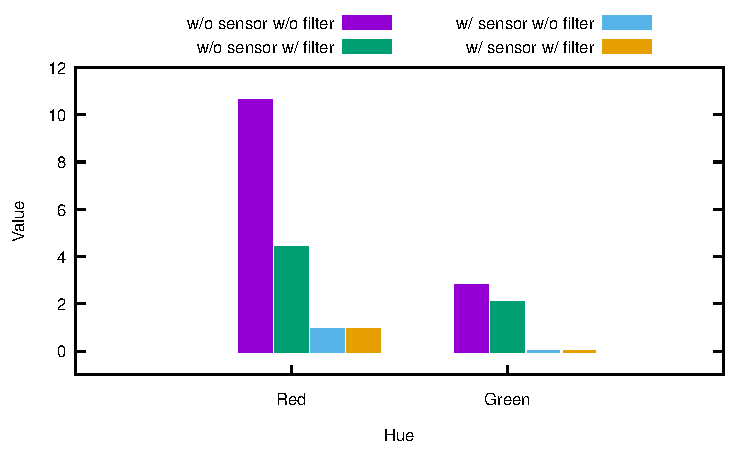
\includegraphics[width=3.1in]{plots/bar_fn.pdf}}
\caption{Misdetection rate for static movement dataset.}
\label{f:fp_stat}
\end{figure}

\ref{t:acc_stat} shows the accuracy rate for the static movement dataset.
It shows that the accuracy increases from 89\% to 97\%.

\begin{table}[h!]
  \centering
  \caption{Accuracy for detection.}
  \label{t:acc_stat}
  \begin{tabular}{  l  c | r  }
   
     & without sensor & with sensor  \\
    \hline
    & 89.7313\% & 97.035\%  \\
    \hline
  \end{tabular}
\end{table}


\section{Evaluation for a public dataset}

\todo{need to add results here}

\section{Effect of video/image resolution}

\ref{f:vf_res} shows the computation time after changing video frames resolution.

\begin{figure}[h!]
  \centering
  \vspace{2in}
  %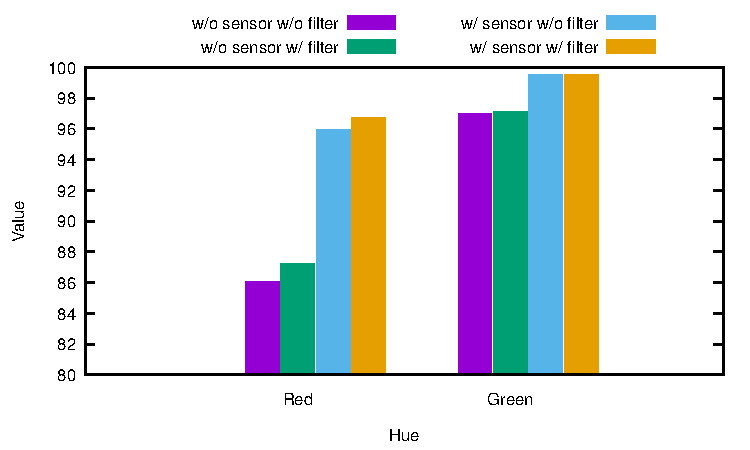
\includegraphics[width=5.2in]{plots/bar_tp.pdf}
  \caption{Effect of the computation time after changing video frames resolution.}
  \label{f:vf_res}
\end{figure}

